\chapter[Coordinate Transformation]{Coordinate Transformation, Contragredient Principle, and Congruent Transformation}
\label{ch:transform}

\section{Coordinate transformation}
\begin{fig}
  % Vector P in two coordinate systems xyz and x'y'z'
\begin{tikzpicture}[scale=1.0,font=\small]
  \coordinate (O) at (0,0);
  \draw[->,thick] (O) -- (3.2,0) node[right] {$x$};
  \draw[->,thick] (O) -- (0,2.6) node[above] {$y$};
  \draw[->,thick] (O) -- (-1.4,-1.4) node[below left] {$z$};
  \draw[->,dashed,thick] (O) -- (2.6,2.0) node[above right] {$x'$};
  \draw[->,dashed,thick] (O) -- (-1.5,2.0) node[above left] {$y'$};
  \draw[->,dashed,thick] (O) -- (-0.2,-1.8) node[below] {$z'$};
  \draw[-{Latex[length=3mm]},line width=1.6pt] (0.6,1.0) -- (1.5,2.1) node[above right] {$\mat{P}$};
\end{tikzpicture}

\end{fig}
The components of a vector in two coordinate systems $xyz$ and $x'y'z'$ have the following relation:
\begin{equation}
  \Bmat{P_{x'}\\ P_{y'}\\ P_{z'}} = \bmat{\lambda_{x'} & \mu_{x'} & \nu_{x'}\\ \lambda_{y'} & \mu_{y'} & \nu_{y'}\\ \lambda_{z'} & \mu_{z'} & \nu_{z'}}\Bmat{P_x\\ P_y\\ P_z}
  \quad\text{or}\quad
  \Bmat{P_x\\ P_y\\ P_z} = \bmat{\lambda_{x'} & \lambda_{y'} & \lambda_{z'}\\ \mu_{x'} & \mu_{y'} & \mu_{z'}\\ \nu_{x'} & \nu_{y'} & \nu_{z'}}\Bmat{P_{x'}\\ P_{y'}\\ P_{z'}}
\end{equation}
i.e.
\begin{equation}
  \Pvec' = \mat{R}\Pvec \quad\text{or}\quad \Pvec = \mat{R}^\tr\Pvec'
\end{equation}
where $\mat{R}$ is a rotation matrix, consisting of the directional cosines of $x'$, $y'$, and $z'$ with respect to the $xyz$ system; namely $\lambda_{x'}^2+\mu_{x'}^2+\nu_{x'}^2 = 1$ and similar expressions for the directional cosines of the $y'$ and $z'$ axes. $\mat{R}$ is orthogonal because $\mat{R}\mat{R}^\tr = \mat{I}$ or equivalently $\mat{R}^{-1} = \mat{R}^\tr$.
\begin{equation}
  \begin{aligned}
    \Pvec &= P_{x'}\mat{i}' + P_{y'}\mat{j}' + P_{z'}\mat{k}'\\
          &= P_{x'}(\lambda_{x'}\mat{i}+\mu_{x'}\mat{j}+\nu_{x'}\mat{k}) + P_{y'}(\lambda_{y'}\mat{i}+\mu_{y'}\mat{j}+\nu_{y'}\mat{k}) + P_{z'}(\lambda_{z'}\mat{i}+\mu_{z'}\mat{j}+\nu_{z'}\mat{k})\\
          &= (P_{x'}\lambda_{x'}+P_{y'}\lambda_{y'}+P_{z'}\lambda_{z'})\mat{i} + (P_{x'}\mu_{x'}+P_{y'}\mu_{y'}+P_{z'}\mu_{z'})\mat{j} + (P_{x'}\nu_{x'}+P_{y'}\nu_{y'}+P_{z'}\nu_{z'})\mat{k}\\
          &= P_x\mat{i} + P_y\mat{j} + P_z\mat{k}
  \end{aligned}
\end{equation}
That is,
\begin{equation}
  \Bmat{P_x\\ P_y\\ P_z} = \bmat{\lambda_{x'} & \lambda_{y'} & \lambda_{z'}\\ \mu_{x'} & \mu_{y'} & \mu_{z'}\\ \nu_{x'} & \nu_{y'} & \nu_{z'}}\Bmat{P_{x'}\\ P_{y'}\\ P_{z'}}
  \qquad\text{or}\qquad \Pvec = \mat{R}^\tr\Pvec'.
\end{equation}

Let the $x'y'z'$ system represent the local (member) coordinate system, and assume that the force--displacement relation for a 3D beam-column element is of the form:
\begin{equation}
  \F' = \Bmat{F_{x'1}\\ F_{y'1}\\ F_{z'1}\\ M_{x'1}\\ M_{y'1}\\ M_{z'1}\\ F_{x'2}\\ F_{y'2}\\ F_{z'2}\\ M_{x'2}\\ M_{y'2}\\ M_{z'2}}
  = \kmat'\Bmat{u_1'\\ v_1'\\ w_1'\\ \theta_{x'1}\\ \theta_{y'1}\\ \theta_{z'1}\\ u_2'\\ v_2'\\ w_2'\\ \theta_{x'2}\\ \theta_{y'2}\\ \theta_{z'2}} = \kmat'\bs{\Delta}'
\end{equation}
where the stiffness matrix in the local axes has been given in Ch.~\ref{ch:beamcolumn} and is not repeated here.

The components of the forces and moments at nodes 1 and 2 in the local coordinate system are related to their components in the global coordinate ($xyz$) system as follows:
\begin{equation}
  \F' = \bmat{\mat{R} & & & \\ & \mat{R} & & \\ & & \mat{R} & \\ & & & \mat{R}}\F = \Tmat\F
\end{equation}
This is because both nodal forces and moments are vectors. Similarly, the nodal degrees of freedom follow the same transformation; that is,
\begin{equation}
  \bs{\Delta}' = \bmat{\mat{R} & & & \\ & \mat{R} & & \\ & & \mat{R} & \\ & & & \mat{R}}\bs{\Delta} = \Tmat\bs{\Delta}
\end{equation}
With the above two transformations, the force--displacement relation becomes:
\begin{equation}
  \F' = \kmat'\bs{\Delta}' \quad\Longrightarrow\quad \Tmat\F = \kmat'\Tmat\bs{\Delta}
\end{equation}
Therefore, we can obtain the force--displacement relation w.r.t.\ the global coordinate system as follows:
\begin{equation}
  \boxed{\F = \Tmat^{-1}\kmat'\Tmat\bs{\Delta} = \Tmat^\tr\kmat'\Tmat\bs{\Delta} = \kmat\bs{\Delta}}
\end{equation}
Note that use has been made of the fact that $\Tmat^{-1} = \Tmat^\tr$ in the derivation of the stiffness transformation; $\kmat = \Tmat^\tr\kmat'\Tmat$. This relation looks very nice and seems familiar to us. Actually, we can see similar transformations in the transformation of stress or strain components, moments of inertia, etc.

\section{Contragredient principle and congruent transformation}
In deriving the stiffness transformation, $\kmat = \Tmat^\tr\kmat'\Tmat$, we have used the fact that $\Tmat^{-1} = \Tmat^\tr$, which holds only when $\Tmat$ is a square matrix. However, the stiffness transformation actually holds even when $\Tmat$ is a rectangular matrix.

Let a structure system (or a member) be described by two pairs of forces and displacements; one consists of $\F$ and $\bs{\Delta}$ and the other $\F'$ and $\bs{\Delta}'$. Usually we say $\F$ and $\bs{\Delta}$ are \emph{work conjugate} to each other and similarly $\F'$ and $\bs{\Delta}'$ are also a work conjugate pair.

The \textbf{contragredient principle} states that
\begin{equation}
  \bs{\Delta}' = \Tmat\bs{\Delta} \quad\Longleftrightarrow\quad \F = \Tmat^\tr\F'
\end{equation}
To prove this principle, we shall know that the strain energy can be written in terms of the two work conjugate pairs as follows.
\begin{equation}
  U = \tfrac12\bs{\Delta}^\tr\F = \tfrac12\bs{\Delta}'^\tr\F'
\end{equation}
Substituting $\bs{\Delta}' = \Tmat\bs{\Delta}$ into the expression for $U$ yields
\begin{equation}
  U = \tfrac12\bs{\Delta}^\tr\F = \tfrac12(\Tmat\bs{\Delta})^\tr\F' = \tfrac12\bs{\Delta}^\tr\Tmat^\tr\F'
\end{equation}
Obviously, $\F = \Tmat^\tr\F'$. Analogously, it is easy to show that if $\F = \Tmat^\tr\F'$, then $\bs{\Delta}' = \Tmat\bs{\Delta}$.

What the contragredient principle says is that once the relation between two force (displacement) vectors is known, then the relation between their conjugate displacement (force) vectors is also sure.

Now assume that the force--displacement relations for the two conjugate pairs are as follows.
\begin{equation}
  \F = \kmat\bs{\Delta},\qquad \F' = \kmat'\bs{\Delta}'
\end{equation}
Then, the strain energy can be written as
\begin{equation}
  U = \tfrac12\bs{\Delta}^\tr\kmat\bs{\Delta} = \tfrac12\bs{\Delta}'^\tr\kmat'\bs{\Delta}'
\end{equation}
Substituting $\bs{\Delta}' = \Tmat\bs{\Delta}$ into the above equation, we can show that
\begin{equation}
  \kmat = \Tmat^\tr\kmat'\Tmat
\end{equation}
This is the so-called \textbf{congruent transformation}.

Note that it is not required that $\Tmat$ be a square and orthogonal matrix when the contragredient principle and the congruent transformation are derived as shown above.

There are various applications of the contragredient principle and congruent transformation. They are not only applicable for a member but also for a structural system. The latter applications include such subjects as static condensation, structures with constraints, and structures with skew supports, which are to be discussed in Ch.~\ref{ch:special}. For the former applications, three examples are provided herein.

\begin{example}
Consider a 2D truss element; its stiffness matrix referred to the member (local) axes is known as:
\begin{equation*}
  \kmat' = \frac{EA}{L}\bmat{1 & -1\\ -1 & 1}
\end{equation*}
Let the local axes $x'$, $y'$ be obtained by rotating counterclockwise the global axes $x$, $y$ an angle $\phi$. Then the displacement vectors in the local and global coordinate systems have the following relation.
\begin{equation*}
  \bs{\Delta}' = \Bmat{u_1'\\ u_2'} = \bmat{\cos\phi & \sin\phi & 0 & 0\\ 0 & 0 & \cos\phi & \sin\phi}\Bmat{u_1\\ v_1\\ u_2\\ v_2} = \Tmat\bs{\Delta}
\end{equation*}
According to the contragredient principle, we obtain
\begin{equation*}
  \F = \Bmat{F_{x1}\\ F_{y1}\\ F_{x2}\\ F_{y2}} = \Tmat^\tr\F' = \Bmat{F_{x'1}\cos\phi\\ F_{x'1}\sin\phi\\ F_{x'2}\cos\phi\\ F_{x'2}\sin\phi}
\end{equation*}
This relation is obviously true.

The stiffness matrix associated with $\bs{\Delta}$ can be obtained through the congruent transformation as follows.
\begin{equation*}
  \kmat = \Tmat^\tr\kmat'\Tmat = \frac{EA}{L}\bmat{c^2 & sc & -c^2 & -sc\\ sc & s^2 & -sc & -s^2\\ -c^2 & -sc & c^2 & sc\\ -sc & -s^2 & sc & s^2}
\end{equation*}
where $c = \cos\phi$ and $s = \sin\phi$.
\end{example}

\begin{example}[Derive {$[k]$} of an unsupported element from {$[k]$} of a supported element]
Considering a simply-supported beam subjected to end moments $M_1$ and $M_2$, these two end moments can be expressed in terms of the corresponding end rotations as:
\begin{fig}
  % Simply supported beam with end moments M1(alpha1), M2(alpha2)
\begin{tikzpicture}[scale=1.1,>=Latex]
  \def\L{6}
  % beam
  \draw[line width=2.2pt,black!70] (0,0) -- (\L,0);
  \node[above] at (\L/2,0.05) {$EI$};
  % pin support (left)
  \draw[fill=black!60] (0,0) -- (-0.25,-0.4) -- (0.25,-0.4) -- cycle;
  \fill[white,draw=black] (0,0) circle (0.06);
  \fill[black!25] (-0.4,-0.4) rectangle (0.4,-0.55);
  % roller support (right)
  \draw[fill=black!60] (\L,0) -- (\L-0.25,-0.4) -- (\L+0.25,-0.4) -- cycle;
  \fill[white,draw=black] (\L,0) circle (0.06);
  \draw[fill=white] (\L-0.15,-0.5) circle (0.09);
  \draw[fill=white] (\L+0.15,-0.5) circle (0.09);
  \fill[black!25] (\L-0.4,-0.6) rectangle (\L+0.4,-0.75);
  % end moments
  \draw[->,thick] (-0.05,0.55) arc (150:-30:0.35);
  \node[above] at (0.2,0.75) {$M_1(\alpha_1)$};
  \draw[->,thick] (\L+0.05,0.55) arc (30:210:0.35);
  \node[above] at (\L-0.2,0.75) {$M_2(\alpha_2)$};
  % length dimension
  \draw[<->] (0,-1.1) -- (\L,-1.1) node[midway,fill=white,inner sep=1pt] {$L$};
  \draw (0,-0.85) -- (0,-1.3);
  \draw (\L,-0.85) -- (\L,-1.3);
\end{tikzpicture}

\end{fig}
\begin{equation*}
  \Bmat{M_{z1}\\ M_{z2}} = \frac{2EI_z}{L}\bmat{2 & 1\\ 1 & 2}\Bmat{\alpha_1\\ \alpha_2}
  \qquad\text{or}\qquad \F' = \kmat'\bs{\Delta}'
\end{equation*}
Assume the corresponding unsupported beam has the following force--displacement relation:
\begin{equation*}
  \F = \Bmat{F_{y1}\\ M_{z1}\\ F_{y2}\\ M_{z2}} = \kmat\bs{\Delta} = \kmat\Bmat{v_1\\ \theta_{z1}\\ v_2\\ \theta_{z2}}
\end{equation*}
The contragredient principle and congruent transformation allow us to investigate the relations between these two conjugate pairs. First, from the equilibrium conditions, we have
\begin{fig}
  % Unsupported beam element: end shears and moments
\begin{tikzpicture}[scale=1.0,font=\small]
  \def\L{6}
  \draw[member] (0,0) -- (\L,0);
  \draw[load] (0,0.1) -- (0,1.3) node[above] {$F_{y1}$};
  \draw[load] (\L,0.1) -- (\L,1.3) node[above] {$F_{y2}$};
  \draw[->,thick] (-0.05,-0.4) arc (-100:100:0.4); \node[left] at (-0.4,0) {$M_{z1}$};
  \draw[->,thick] (\L+0.05,-0.4) arc (280:80:0.4); \node[right] at (\L+0.4,0) {$M_{z2}$};
  \draw[dim] (0,-0.9) -- (\L,-0.9) node[midway,fill=white,inner sep=1pt] {$L$};
  \draw (0,-0.7) -- (0,-1.1); \draw (\L,-0.7) -- (\L,-1.1);
\end{tikzpicture}

\end{fig}
\begin{equation*}
  F_{y1} = \frac{M_{z1}+M_{z2}}{L},\quad\text{and}\quad F_{y2} = -\frac{M_{z1}+M_{z2}}{L}
\end{equation*}
\begin{equation*}
  \Bmat{F_{y1}\\ M_{z1}\\ F_{y2}\\ M_{z2}} =
  \begin{bmatrix} \dfrac1L & \dfrac1L\\[6pt] 1 & 0\\[3pt] -\dfrac1L & -\dfrac1L\\[6pt] 0 & 1\end{bmatrix}
  \Bmat{M_{z1}\\ M_{z2}},\quad\text{or}\quad \F = \Tmat^\tr\F'
\end{equation*}
According to the contragredient principle,
\begin{equation*}
  \bs{\Delta}' = \Tmat\bs{\Delta},\quad\text{or}\quad
  \Bmat{\alpha_1\\ \alpha_2} = \begin{bmatrix}\dfrac1L & 1 & -\dfrac1L & 0\\[6pt] \dfrac1L & 0 & -\dfrac1L & 1\end{bmatrix}\Bmat{v_1\\ \theta_{z1}\\ v_2\\ \theta_{z2}}
\end{equation*}
That is,
\begin{equation*}
  \alpha_1 = \theta_{z1}-\theta_r = \theta_{z1}-\frac{v_2-v_1}{L}\quad\text{and}\quad
  \alpha_2 = \theta_{z2}-\theta_r = \theta_{z2}-\frac{v_2-v_1}{L}
\end{equation*}
\begin{fig}
  % End rotations w.r.t. the chord: alpha_i = theta_zi - theta_r
\begin{tikzpicture}[scale=1.0,font=\small]
  \coordinate (A) at (0,0); \coordinate (B) at (9,3);
  % chord
  \draw[very thick] (A) -- (B);
  % deflected shape (dashed)
  \draw[dashed,thick] (A) .. controls (2.5,2.6) and (6.0,1.2) .. (B);
  % tangents at the ends
  \draw[thin] (A) -- ++(52:1.6); \draw[thin] (B) -- ++(232:1.9);
  % horizontal references
  \draw[thin] (A) -- ++(2.2,0); \draw[thin] (B) -- ++(-2.2,0);
  % angles at end 1
  \draw[->] ($(A)+(1.6,0)$) arc (0:18.4:1.6); \node at (1.95,0.25) {$\theta_r$};
  \draw[->] ($(A)+(1.1,0)$) arc (0:52:1.1); \node at (1.05,0.9) {$\theta_{z1}$};
  \draw[->] ($(A)+(18.4:1.4)$) arc (18.4:52:1.4); \node at (1.1,1.35) {$\alpha_1$};
  % angles at end 2
  \draw[->] ($(B)+(180:1.6)$) arc (180:198.4:1.6); \node at ($(B)+(-1.9,-0.25)$) {$\theta_{z2}$};
  \draw[->] ($(B)+(198.4:1.3)$) arc (198.4:232:1.3); \node at ($(B)+(-1.35,-0.95)$) {$\alpha_2$};
  % vertical dims
  \draw[dim] (-0.3,-1.5) -- (-0.3,0) node[midway,left] {$v_1$};
  \draw[dim] (9.3,-1.5) -- (9.3,3) node[midway,right] {$v_2$};
  \draw[thin] (0,-1.5) -- (-0.5,-1.5); \draw[thin] (9,-1.5) -- (9.5,-1.5);
  \draw[dim] (0,-1.5) -- (9,-1.5) node[midway,fill=white,inner sep=1pt] {$L$};
\end{tikzpicture}

\end{fig}
\begin{equation*}
  \begin{aligned}
  M_{12} &= \frac{2EI}{L}\bigl[2\alpha_1+\alpha_2\bigr] = \frac{2EI}{L}\bigl[2(\theta_{z1}-\theta_r)+(\theta_{z2}-\theta_r)\bigr]\\
         &= \frac{2EI}{L}(2\theta_{z1}+\theta_{z2}-3\theta_r) = \frac{2EI}{L}\Bigl(2\theta_{z1}+\theta_{z2}-3\frac{\Delta}{L}\Bigr)
  \end{aligned}
\end{equation*}
where $\theta_r = (v_2-v_1)/L = \Delta/L$ is the rotation of the chord connecting nodes 1 and 2. Therefore, $\alpha_1$ and $\alpha_2$ are the end rotations w.r.t.\ the chord; they are often called \emph{natural deformations} because rigid body displacements are excluded. This is \emph{the slope deflection equation}.

In the above, we first establish the force relations, $\F = \Tmat^\tr\F'$, and then obtain the displacement relations according to the contragredient principle. Of course, we can also reverse the sequence.

The stiffness matrix for the unsupported beam can be obtained through the use of the congruent transformation; hence,
\begin{equation*}
  \kmat = \Tmat^\tr\kmat'\Tmat = \frac{EI_z}{L}
  \begin{bmatrix}
    \dfrac{12}{L^2} & \dfrac6L & -\dfrac{12}{L^2} & \dfrac6L\\[8pt]
    \dfrac6L & 4 & -\dfrac6L & 2\\[8pt]
    -\dfrac{12}{L^2} & -\dfrac6L & \dfrac{12}{L^2} & -\dfrac6L\\[8pt]
    \dfrac6L & 2 & -\dfrac6L & 4
  \end{bmatrix}
\end{equation*}
The result is the same as that derived in Ch.~\ref{ch:beamcolumn}.
\end{example}

\begin{example}
Consider an elastic beam of length $L$ with rigid zones at ends, whose lengths are $a$ (left) and $b$ (right), respectively. Denote the degrees of freedom of the beam with rigid zones by $\bs{\Delta}$ and those of the beam by $\bs{\Delta}'$. Then, it is easy to show that
\begin{fig}
  % Beam with rigid zones: DOFs Delta (with rigid zones) and Delta' (elastic beam only)
\begin{tikzpicture}[scale=0.68,font=\small]
  % ---- with rigid zones ----
  \begin{scope}
    \fill[hatch] (0,-0.12) rectangle (1.0,0.12); \draw (0,-0.12) rectangle (1.0,0.12);
    \draw[member] (1.0,0) -- (5.5,0);
    \fill[hatch] (5.5,-0.12) rectangle (6.2,0.12); \draw (5.5,-0.12) rectangle (6.2,0.12);
    \draw[load] (-1.2,0) -- (-0.1,0) node[pos=0,left] {$u_1$};
    \draw[load] (0,0.15) -- (0,1.2) node[above] {$v_1$};
    \draw[->,thick] (0.35,-0.3) arc (-40:200:0.35); \node[below left] at (0,-0.35) {$\theta_{z1}$};
    \draw[load] (6.3,0) -- (7.4,0) node[right] {$u_2$};
    \draw[load] (6.2,0.15) -- (6.2,1.2) node[above] {$v_2$};
    \draw[->,thick] (6.55,-0.3) arc (-40:200:0.35); \node[below right] at (6.2,-0.35) {$\theta_{z2}$};
    \node[below] at (0.5,-0.15) {$a$}; \node[below] at (5.85,-0.15) {$b$};
    \draw[dim] (1.0,-0.9) -- (5.5,-0.9) node[midway,fill=white,inner sep=1pt] {$L$};
  \end{scope}
  % ---- elastic beam only ----
  \begin{scope}[xshift=10cm]
    \draw[member] (0,0) -- (4.5,0);
    \draw[load] (-1.2,0) -- (-0.1,0) node[pos=0,left] {$u_1'$};
    \draw[load] (0,0.15) -- (0,1.2) node[above] {$v_1'$};
    \draw[->,thick] (0.35,-0.3) arc (-40:200:0.35); \node[below left] at (0,-0.35) {$\theta_{z1}'$};
    \draw[load] (4.6,0) -- (5.7,0) node[right] {$u_2'$};
    \draw[load] (4.5,0.15) -- (4.5,1.2) node[above] {$v_2'$};
    \draw[->,thick] (4.85,-0.3) arc (-40:200:0.35); \node[below right] at (4.5,-0.35) {$\theta_{z2}'$};
    \draw[dim] (0,-0.9) -- (4.5,-0.9) node[midway,fill=white,inner sep=1pt] {$L$};
  \end{scope}
\end{tikzpicture}

\end{fig}
\begin{equation*}
  \bs{\Delta}' = \Bmat{u_1'\\ v_1'\\ \theta_{z1}'\\ u_2'\\ v_2'\\ \theta_{z2}'} =
  \bmat{1 & 0 & 0 & 0 & 0 & 0\\ 0 & 1 & a & 0 & 0 & 0\\ 0 & 0 & 1 & 0 & 0 & 0\\ 0 & 0 & 0 & 1 & 0 & 0\\ 0 & 0 & 0 & 0 & 1 & -b\\ 0 & 0 & 0 & 0 & 0 & 1}
  \Bmat{u_1\\ v_1\\ \theta_{z1}\\ u_2\\ v_2\\ \theta_{z2}} = \Tmat\bs{\Delta}
\end{equation*}
The same $\Tmat$ can also be derived from the conditions, $\F = \Tmat^\tr\F'$.
\begin{fig}
  % Beam with rigid zones: forces F and F'
\begin{tikzpicture}[scale=0.68,font=\small]
  \begin{scope}
    \fill[hatch] (0,-0.12) rectangle (1.0,0.12); \draw (0,-0.12) rectangle (1.0,0.12);
    \draw[member] (1.0,0) -- (5.5,0);
    \fill[hatch] (5.5,-0.12) rectangle (6.2,0.12); \draw (5.5,-0.12) rectangle (6.2,0.12);
    \draw[load] (-1.2,0) -- (-0.1,0) node[pos=0,left] {$F_{x1}$};
    \draw[load] (0,0.15) -- (0,1.2) node[above] {$F_{y1}$};
    \draw[->,thick] (0.35,-0.3) arc (-40:200:0.35); \node[below left] at (0,-0.35) {$M_{z1}$};
    \draw[load] (6.3,0) -- (7.4,0) node[right] {$F_{x2}$};
    \draw[load] (6.2,0.15) -- (6.2,1.2) node[above] {$F_{y2}$};
    \draw[->,thick] (6.55,-0.3) arc (-40:200:0.35); \node[below right] at (6.2,-0.35) {$M_{z2}$};
    \node[below] at (0.5,-0.15) {$a$}; \node[below] at (5.85,-0.15) {$b$};
    \draw[dim] (1.0,-0.9) -- (5.5,-0.9) node[midway,fill=white,inner sep=1pt] {$L$};
  \end{scope}
  \begin{scope}[xshift=10cm]
    \draw[member] (0,0) -- (4.5,0);
    \draw[load] (-1.2,0) -- (-0.1,0) node[pos=0,left] {$F_{x1}$};
    \draw[load] (0,0.15) -- (0,1.2) node[above] {$F_{y1}$};
    \draw[->,thick] (0.35,-0.3) arc (-40:200:0.35); \node[below left,align=right] at (0.1,-0.35) {$M_{z1}-F_{y1}\cdot a$};
    \draw[load] (4.6,0) -- (5.7,0) node[right] {$F_{x2}$};
    \draw[load] (4.5,0.15) -- (4.5,1.2) node[above] {$F_{y2}$};
    \draw[->,thick] (4.85,-0.3) arc (-40:200:0.35); \node[below right] at (4.4,-0.35) {$M_{z2}+F_{y2}\cdot b$};
    \draw[dim] (0,-0.9) -- (4.5,-0.9) node[midway,fill=white,inner sep=1pt] {$L$};
  \end{scope}
\end{tikzpicture}

\end{fig}
Therefore
\begin{equation*}
  \begin{array}{lcl}
    F_{x1}' = F_{x1} & \rightarrow & F_{x1} = F_{x1}'\\
    F_{y1}' = F_{y1} & \rightarrow & F_{y1} = F_{y1}'\\
    M_{z1}' = M_{z1} - F_{y1}a & \rightarrow & M_{z1} = M_{z1}' + F_{y1}a = M_{z1}' + F_{y1}'a\\
    F_{x2}' = F_{x2} & \rightarrow & F_{x2} = F_{x2}'\\
    F_{y2}' = F_{y2} & \rightarrow & F_{y2} = F_{y2}'\\
    M_{z2}' = M_{z2} + F_{y2}b & \rightarrow & M_{z2} = M_{z2}' - F_{y2}b = M_{z2}' - F_{y2}'b
  \end{array}
\end{equation*}
In matrix form,
\begin{equation*}
  \F = \Bmat{F_{x1}\\ F_{y1}\\ M_{z1}\\ F_{x2}\\ F_{y2}\\ M_{z2}} =
  \bmat{1 & 0 & 0 & 0 & 0 & 0\\ 0 & 1 & 0 & 0 & 0 & 0\\ 0 & a & 1 & 0 & 0 & 0\\ 0 & 0 & 0 & 1 & 0 & 0\\ 0 & 0 & 0 & 0 & 1 & 0\\ 0 & 0 & 0 & 0 & -b & 1}
  \Bmat{F_{x1}'\\ F_{y1}'\\ M_{z1}'\\ F_{x2}'\\ F_{y2}'\\ M_{z2}'} = \Tmat^\tr\F'
\end{equation*}
The stiffness matrix for the beam with rigid zones, $\kmat$, can then be related to the stiffness matrix of the beam without rigid zones, $\kmat'$, through the congruent transformation; that is
\begin{equation*}
  \kmat = \Tmat^\tr\kmat'\Tmat
\end{equation*}
\end{example}

\begin{example}
Consider an elastic beam of length $L$ connecting an axial force member by two rigid links, whose lengths are $e_1$ (left) and $e_2$ (right). The axial force member has the axial rigidity of $EA$ and length of $L_1$, where $L_1 = \sqrt{L^2+(e_2-e_1)^2}$.
\begin{fig}
  % Beam connected to an axial member by two rigid links
\begin{tikzpicture}[scale=0.68,font=\small]
  % ---- (a) DOF Delta ----
  \begin{scope}
    \draw[fill=black!15] (0,0) rectangle (5.5,0.3);
    \node[above] at (2.75,0.3) {$E, I, A, L$};
    \fill[hatch] (0,-0.5) rectangle (0.18,0); \draw (0,-0.5) rectangle (0.18,0);
    \fill[hatch] (5.32,-0.9) rectangle (5.5,0); \draw (5.32,-0.9) rectangle (5.5,0);
    \draw[thinmember] (0.09,-0.5) -- (5.41,-0.9);
    \node[below] at (2.75,-0.75) {$E, A, L_1$};
    \node[right,font=\footnotesize] at (0.2,-0.25) {$e_1$}; \node[left,font=\footnotesize] at (5.3,-0.45) {$e_2$};
    \node[below left] at (0,0) {1}; \node[below right] at (5.5,0) {2};
    \draw[load] (-1.2,0.15) -- (-0.1,0.15) node[pos=0,left] {$u_1$};
    \draw[load] (0,0.4) -- (0,1.4) node[above] {$v_1$};
    \draw[->,thick] (0.3,-0.1) arc (-30:200:0.35); \node[below left] at (-0.1,-0.35) {$\theta_{z1}$};
    \draw[load] (5.6,0.15) -- (6.7,0.15) node[right] {$u_2$};
    \draw[load] (5.5,0.4) -- (5.5,1.4) node[above] {$v_2$};
    \draw[->,thick] (5.8,-0.1) arc (-30:200:0.35); \node[below right] at (5.6,-0.35) {$\theta_{z2}$};
    \node[below] at (2.75,-1.7) {(a) Degrees of freedom $\bs{\Delta}$};
  \end{scope}
  % ---- (b) DOF Delta' ----
  \begin{scope}[xshift=9.5cm]
    \draw[thinmember] (0,-0.5) -- (5.5,-0.9);
    \node[below] at (2.75,-0.85) {$E, A, L_1$};
    \draw[load] (-1.2,-0.5) -- (-0.1,-0.5) node[pos=0,left] {$d_1$};
    \draw[load] (0,-0.4) -- (0,0.8) node[above] {$d_2$};
    \draw[load] (5.6,-0.9) -- (6.7,-0.9) node[right] {$d_3$};
    \draw[load] (5.5,-0.8) -- (5.5,0.4) node[above] {$d_4$};
    \node[below] at (2.75,-1.7) {(b) Degrees of freedom $\bs{\Delta}'$};
  \end{scope}
\end{tikzpicture}

\end{fig}
The strain energy of the system is
\begin{equation*}
  U = U_b + U_{truss} = \tfrac12\bs{\Delta}^\tr\kmat_b\bs{\Delta} + \tfrac12\bs{\Delta}^\tr\kmat_t\bs{\Delta}
  \quad\Longrightarrow\quad \kmat = \kmat_b + \kmat_t
\end{equation*}
The stiffness matrix of the truss $\kmat'$ corresponding to $\bs{\Delta}'$ is known, but what is the stiffness matrix of the truss corresponding to $\bs{\Delta}$? This can be easily done with the aid of the congruent transformation. It is not difficult to show that
\begin{equation*}
  \bs{\Delta}' = \Bmat{d_1\\ d_2\\ d_3\\ d_4} =
  \bmat{1 & 0 & e_1 & 0 & 0 & 0\\ 0 & 1 & 0 & 0 & 0 & 0\\ 0 & 0 & 0 & 1 & 0 & e_2\\ 0 & 0 & 0 & 0 & 1 & 0}
  \Bmat{u_1\\ v_1\\ \theta_1\\ u_2\\ v_2\\ \theta_2},\quad\text{or}\quad \bs{\Delta}' = \Tmat\bs{\Delta}.
\end{equation*}
Then, according to the congruent transformation $\kmat_t = \Tmat^\tr\kmat'\Tmat$, we have
\begin{equation*}
  \kmat_t = \frac{EA}{L_1}
  \begin{bmatrix}
    c^2 & sc & e_1c^2 & -c^2 & -sc & -e_2c^2\\
    sc & s^2 & e_1sc & -sc & -s^2 & -e_2sc\\
    e_1c^2 & e_1sc & e_1^2c^2 & -e_1c^2 & -e_1sc & -e_1e_2c^2\\
    -c^2 & -sc & -e_1c^2 & c^2 & sc & e_2c^2\\
    -sc & -s^2 & -e_1sc & sc & s^2 & e_2sc\\
    -e_2c^2 & -e_2sc & -e_1e_2c^2 & e_2c^2 & e_2sc & e_2^2c^2
  \end{bmatrix}
\end{equation*}
The same result can be obtained if two degrees of freedom along the member axis are used for the axial force member. Try it.
\end{example}

\begin{example}
Use the congruent transformation to derive the stiffness matrix for a beam element bent about the $y$-axis from that bent about the $z$-axis.
\begin{equation*}
  \kmat_y = \frac{EI_y}{L}
  \begin{bmatrix}
    \dfrac{12}{L^2} & -\dfrac6L & -\dfrac{12}{L^2} & -\dfrac6L\\[8pt]
    -\dfrac6L & 4 & \dfrac6L & 2\\[8pt]
    -\dfrac{12}{L^2} & \dfrac6L & \dfrac{12}{L^2} & \dfrac6L\\[8pt]
    -\dfrac6L & 2 & \dfrac6L & 4
  \end{bmatrix}\Bmat{w_1\\ \theta_{y1}\\ w_2\\ \theta_{y2}};\qquad
  \kmat_z = \frac{EI_z}{L}
  \begin{bmatrix}
    \dfrac{12}{L^2} & \dfrac6L & -\dfrac{12}{L^2} & \dfrac6L\\[8pt]
    \dfrac6L & 4 & -\dfrac6L & 2\\[8pt]
    -\dfrac{12}{L^2} & -\dfrac6L & \dfrac{12}{L^2} & -\dfrac6L\\[8pt]
    \dfrac6L & 2 & -\dfrac6L & 4
  \end{bmatrix}
\end{equation*}
\begin{equation*}
  \kmat_y = \Tmat^\tr\kmat_z\Tmat;\qquad \Tmat = ?
\end{equation*}
\end{example}

\section{Transformation matrices for all types of framed elements in FRAME21}
\begin{enumerate}[leftmargin=*]
  \item \underline{Beam element, \texttt{ITP}=1 (lies in the $x$-$y$ plane)}\\
    Degrees of freedom: $\bs{\Delta}^\tr = \langle v_1, \theta_{z1}, v_2, \theta_{z2}\rangle = \langle 2, 6, 8, 12\rangle$
    \begin{equation*}
      \Tmat = \bmat{\mat{R} & \\ & \mat{R}} = \mat{I}_{4\times4},\quad\text{with } \mat{R} = \mat{I}_{2\times2}.
    \end{equation*}

  \item \underline{2D truss element, \texttt{ITP}=2 (lies in the $x$-$y$ plane)}\\
    Degrees of freedom: $\bs{\Delta}^\tr = \langle u_1, v_1, u_2, v_2\rangle = \langle 1, 2, 7, 8\rangle$
    \begin{equation*}
      \Tmat = \bmat{\mat{R} & \\ & \mat{R}},\quad\text{with } \mat{R} = \bmat{\cos\phi & \sin\phi\\ -\sin\phi & \cos\phi}
    \end{equation*}
    where $\cos\phi = \dfrac{x_2-x_1}{L}$, $\sin\phi = \dfrac{y_2-y_1}{L}$. Note that
    $\kmat' = \dfrac{EA}{L}\bmat{1 & 0 & -1 & 0\\ 0 & 0 & 0 & 0\\ -1 & 0 & 1 & 0\\ 0 & 0 & 0 & 0}$.

  \item \underline{2D frame element, \texttt{ITP}=3 (lies in the $x$-$y$ plane)}\\
    Degrees of freedom: $\bs{\Delta}^\tr = \langle u_1, v_1, \theta_{z1}, u_2, v_2, \theta_{z2}\rangle = \langle 1, 2, 6, 7, 8, 12\rangle$
    \begin{equation*}
      \Tmat = \bmat{\mat{R} & \\ & \mat{R}},\quad\text{with } \mat{R} = \bmat{\cos\phi & \sin\phi & 0\\ -\sin\phi & \cos\phi & 0\\ 0 & 0 & 1}
    \end{equation*}

  \item \underline{Grid element, \texttt{ITP}=4 (lies in the $x$-$z$ plane)}\\
    \begin{minipage}[t]{0.6\linewidth}
      Degrees of freedom:
      $\bs{\Delta}^\tr = \langle v_1, \theta_{x1}, \theta_{z1}, v_2, \theta_{x2}, \theta_{z2}\rangle = \langle 2, 4, 6, 8, 10, 12\rangle$
      \begin{enumerate}[label=(\arabic*)]
        \item bend about the strong ($z$-) axis.
        \item can take torsion.
      \end{enumerate}
    \end{minipage}\hfill
    \begin{minipage}[t]{0.36\linewidth}
      \vspace{0pt}\centering% Grid element (ITP=4) lying in the x-z plane
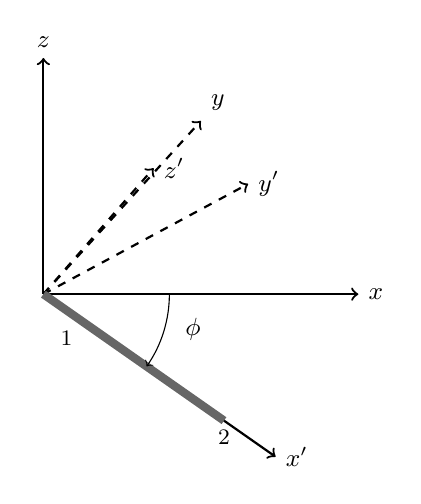
\begin{tikzpicture}[scale=1.0,font=\small]
  \coordinate (O) at (0,0);
  \draw[->,thick] (O) -- (0,3.0) node[above] {$z$};
  \draw[->,thick] (O) -- (4.0,0) node[right] {$x$};
  \draw[->,dashed,thick] (O) -- (2.0,2.2) node[above right] {$y$};
  \draw[->,dashed,thick] (O) -- (1.4,1.6) node[right] {$z'$};
  \draw[->,dashed,thick] (O) -- (2.6,1.4) node[right] {$y'$};
  % member along x'
  \draw[line width=3pt,black!60] (O) -- (-35:2.8);
  \draw[->,thick] (-35:2.8) -- (-35:3.6) node[right] {$x'$};
  \node[below left,font=\footnotesize] at (-35:0.6) {1}; \node[below,font=\footnotesize] at (-35:2.8) {2};
  \draw[->] (1.6,0) arc (0:-35:1.6); \node at (1.9,-0.45) {$\phi$};
\end{tikzpicture}

    \end{minipage}
    \begin{equation*}
      \bs{\Delta}' = \Bmat{v_1'\\ \theta_{x1}'\\ \theta_{z1}'\\ v_2'\\ \theta_{x2}'\\ \theta_{z2}'} = \Tmat\bs{\Delta} = \Tmat\Bmat{v_1\\ \theta_{x1}\\ \theta_{z1}\\ v_2\\ \theta_{x2}\\ \theta_{z2}}
    \end{equation*}
    where $\Tmat = \bmat{\mat{R} & \\ & \mat{R}}$, and $\mat{R} = \bmat{1 & 0 & 0\\ 0 & \cos\phi & -\sin\phi\\ 0 & \sin\phi & \cos\phi}$. The values of $\sin\phi$ and $\cos\phi$ can be evaluated by
    \begin{equation*}
      \cos\phi = \frac{x_2-x_1}{L},\qquad \sin\phi = -\frac{z_2-z_1}{L}\quad\text{(different from 2D truss)}
    \end{equation*}

    \begin{example}[Grid structure; Sack (1989), \emph{Matrix Structural Analysis}, pp.~198--200, Example~5.4]
    Analyze the simple grid shown below. For all elements $I_y = 350$~in$^4$, $I_z = 700$~in$^4$; $J = 800$~in$^4$; $E = 29\times10^3$~kips/in$^2$; and $G = 11\times10^3$~kips/in$^2$.
    \begin{fig}
      % Simple grid (after Sack, 1989, Example 5.4): grid with loading (isometric sketch)
\begin{tikzpicture}[scale=0.9,font=\footnotesize,x={(1cm,0cm)},y={(0cm,1cm)},z={(-0.55cm,-0.42cm)}]
  \coordinate (a) at (0,0,0);
  \coordinate (b) at (4.5,0,0); \coordinate (d) at (-3.6,0,0);
  \coordinate (e) at (0,0,-3.6); \coordinate (c) at (0,0,5.0);
  % members
  \draw[line width=2.4pt,black!65] (d) -- (b);
  \draw[line width=2.4pt,black!65] (e) -- (c);
  % fixed ends
  \foreach \p in {b,d}{\fill[hatch] ($(\p)+(-0.15,-0.25,0)$) -- ($(\p)+(0.15,-0.25,0)$) -- ($(\p)+(0.15,0.55,0)$) -- ($(\p)+(-0.15,0.55,0)$) -- cycle;}
  \foreach \p in {e,c}{\fill[hatch] ($(\p)+(0,-0.25,-0.15)$) -- ($(\p)+(0,-0.25,0.15)$) -- ($(\p)+(0,0.55,0.15)$) -- ($(\p)+(0,0.55,-0.15)$) -- cycle;}
  % distributed load on ad
  \foreach \t in {0.12,0.3,...,0.95}{\draw[->] (-3.6*\t,1.0,0) -- (-3.6*\t,0.1,0);}
  \draw (-3.6*0.12,1.0,0) -- (-3.6*0.95,1.0,0);
  \node[above] at (-1.9,1.0,0) {10 k/ft};
  % distributed load on ac
  \foreach \t in {0.1,0.22,...,0.95}{\draw[->] (0,1.0,5.0*\t) -- (0,0.1,5.0*\t);}
  \draw (0,1.0,5.0*0.1) -- (0,1.0,5.0*0.95);
  \node[left] at (0,1.15,3.0) {10 k/ft};
  % node labels
  \node[above right] at (a) {$a$}; \node[above] at ($(b)+(0,0.6,0)$) {$b$}; \node[right] at ($(c)+(0.2,0,0)$) {$c$};
  \node[above] at ($(d)+(0,0.6,0)$) {$d$}; \node[above] at ($(e)+(0,0.6,0)$) {$e$};
  % axes
  \draw[->] (a) -- (0,2.2,0) node[above] {$y$};
  \draw[->] ($(b)+(0.3,0,0)$) -- (6.0,0,0) node[right] {$x$};
  \draw[->] ($(c)+(0,0,0.3)$) -- (0,0,6.6) node[below left] {$z$};
  % dimensions (below the members)
  \node[below,inner sep=5pt] at (2.25,0,0) {18 ft}; \node[below,inner sep=5pt] at (-1.8,0,0) {12 ft};
  \node[right,inner sep=5pt] at (0,0,2.6) {20 ft}; \node[right,inner sep=5pt] at (0,0,-1.9) {12 ft};
\end{tikzpicture}

    \end{fig}
    \begin{solution}
    The element stiffness matrices are obtained using Eq.~(5.37) of Sack. Assuming axial inextensibility of all elements, we need consider only $V_a$, $\Theta_{xa}$, and $\Theta_{za}$. Note that this simplifies calculation of relevant element stiffness entries (we urge the reader to calculate the appropriate 3 by 3 partition for the four element stiffness matrices). Invoking nodal equilibrium for the structure with support conditions enforced yields (the reader is encouraged to carry out this process)
    \begin{equation*}
      \Bmat{-160\\ 4000\\ 1440} = \bmat{264.35 & 6343.8 & -3263.2\\ 6343.8 & 1116900 & 00000\\ -3263.2 & 00000 & 1049800}\Bmat{V_a\\ \Theta_{xa}\\ \Theta_{za}}
    \end{equation*}
    (with forces in kips and moments in kip$\cdot$in). Hence
    \begin{equation*}
      \Bmat{V_a\\ \Theta_{xa}\\ \Theta_{za}} = \Bmat{-0.8170\text{ in.}\\ 8.222\times10^{-3}\text{ rad}\\ -1.168\times10^{-3}\text{ rad}}
    \end{equation*}
    For elements $ab$ and $ae$ the element forces are obtained using Eq.~(5.42) of Sack; thus
    \begin{equation*}
      \Bmat{\bar p_{\bar ya}\\ \bar m_{\bar xa}\\ \bar m_{\bar za}\\ \bar m_{\bar zb}}^{ab} = \mat{e}\mat{u}^{ab} = \Bmat{-22.8\text{ kips}\\ +335\text{ kip}\cdot\text{in.}\\ -2570\text{ kip}\cdot\text{in.}\\ -2350\text{ kip}\cdot\text{in.}}
      \quad\text{and}\quad
      \Bmat{\bar p_{\bar ya}\\ \bar m_{\bar xa}\\ \bar m_{\bar za}\\ \bar m_{\bar ze}}^{ae} = \mat{e}\mat{u}^{ae} = \Bmat{-45.6\text{ kips}\\ +85.6\text{ kip}\cdot\text{in.}\\ -1350\text{ kip}\cdot\text{in.}\\ -4130\text{ kip}\cdot\text{in.}}
    \end{equation*}
    Elements $ac$ and $ad$ have initial forces applied; therefore using Eq.~(4.65) of Sack we have
    \begin{equation*}
      \Bmat{\bar p_{\bar ya}\\ \bar p_{\bar yc}\\ \bar m_{\bar xa}\\ \bar m_{\bar za}\\ \bar m_{\bar zc}}^{ac} = \mat{e}\mat{u}^{ac}+\bar{\mat{s}}^o
      = \Bmat{-31.8\\ +31.8\\ 42.8\\ -4510\\ -3120} + \Bmat{100\\ 100\\ 0\\ 4000\\ -4000}
      = \Bmat{68.2\text{ kips}\\ 131.8\text{ kips}\\ -42.8\text{ kip}\cdot\text{in.}\\ -510\text{ kip}\cdot\text{in.}\\ -7120\text{ kip}\cdot\text{in.}}
    \end{equation*}
    and
    \begin{equation*}
      \Bmat{\bar p_{\bar ya}\\ \bar p_{\bar yd}\\ \bar m_{\bar xa}\\ \bar m_{\bar za}\\ \bar m_{\bar zd}}^{ad} = \mat{e}\mat{u}^{ad}+\bar{\mat{s}}^o
      = \Bmat{-59.8\\ +59.8\\ -502\\ -4140\\ 4470} + \Bmat{60\\ 60\\ 0\\ 1440\\ -1440}
      = \Bmat{+0.2\text{ kips}\\ 119.8\text{ kips}\\ -502\text{ kip}\cdot\text{in.}\\ -2700\text{ kip}\cdot\text{in.}\\ -5910\text{ kip}\cdot\text{in.}}
    \end{equation*}
    \begin{figure}[H]
      \centering
      % Free-body diagrams of the grid members and node a, drawn in plan view
% (forces in kips, moments in kip-in).  Vertical (y) forces: dot = up (+y), cross = down.
% Double-headed arrows = moment vectors (about x or z).
\begin{tikzpicture}[scale=0.8,font=\scriptsize,
  mom/.style={->,thick,double,double distance=1pt},
  up/.pic={\draw[fill=white] (0,0) circle (0.13); \fill (0,0) circle (0.04);},
  down/.pic={\draw[fill=white] (0,0) circle (0.13); \draw (-0.09,-0.09) -- (0.09,0.09); \draw (-0.09,0.09) -- (0.09,-0.09);}]
  % plan: x to the right, z downwards on the page
  \draw[->] (-7.2,3.6) -- (-6.2,3.6) node[right] {$x$}; \draw[->] (-7.2,3.6) -- (-7.2,2.6) node[below] {$z$};
  % ---------------- node a ----------------
  \draw[line width=1.5pt] (-0.5,0) -- (0.5,0); \draw[line width=1.5pt] (0,-0.5) -- (0,0.5);
  \fill (0,0) circle (0.05); \node[above left] at (0,0) {$a$};
  % from ab (right)
  \pic at (1.4,-0.5) {up}; \node[below] at (1.4,-0.65) {22.8};
  \draw[mom] (0.6,0) -- (2.0,0) node[right] {335};
  \draw[mom] (1.4,0.25) -- (1.4,1.3) node[above] {2570};
  % from ad (left)
  \pic at (-1.4,-0.5) {down}; \node[below] at (-1.4,-0.65) {0.2};
  \draw[mom] (-0.6,0) -- (-2.0,0) node[left] {502};
  \draw[mom] (-1.4,0.25) -- (-1.4,1.3) node[above] {2700};
  % from ae (top, -z)
  \pic at (-0.5,1.9) {up}; \node[left] at (-0.65,1.9) {45.6};
  \draw[mom] (0,0.6) -- (0,2.4) node[above] {85.6};
  \draw[mom] (0.25,2.1) -- (1.4,2.1) node[right] {1350};
  % from ac (bottom, +z)
  \pic at (-0.5,-1.9) {down}; \node[left] at (-0.65,-1.9) {68.2};
  \draw[mom] (0,-0.6) -- (0,-2.4) node[below] {42.8};
  \draw[mom] (0.25,-2.1) -- (1.4,-2.1) node[right] {510};
  % ---------------- member ab ----------------
  \begin{scope}[shift={(4.8,0)}]
    \draw[line width=1.5pt,black!70] (0,0) -- (3.4,0); \node[below] at (1.7,-0.1) {$ab$};
    \pic at (0,0.45) {down}; \node[above] at (0,0.6) {22.8};
    \draw[mom] (-0.15,0) -- (-1.0,0) node[left] {335};
    \draw[mom] (0.3,-0.2) -- (0.3,-1.0) node[below] {2570};
    \pic at (3.4,0.45) {up}; \node[above] at (3.4,0.6) {22.8};
    \draw[mom] (3.55,0) -- (4.4,0) node[right] {335};
    \draw[mom] (3.1,-0.2) -- (3.1,-1.0) node[below] {2350};
  \end{scope}
  % ---------------- member ad ----------------
  \begin{scope}[shift={(-4.8,0)}]
    \draw[line width=1.5pt,black!70] (0,0) -- (-3.4,0); \node[below] at (-1.7,-0.1) {$ad$};
    \pic at (0,0.45) {up}; \node[above] at (0,0.6) {0.2};
    \draw[mom] (0.15,0) -- (1.0,0) node[right] {502};
    \draw[mom] (-0.3,-0.2) -- (-0.3,-1.0) node[below] {2700};
    \pic at (-3.4,0.45) {up}; \node[above] at (-3.4,0.6) {119.8};
    \draw[mom] (-3.55,0) -- (-4.4,0) node[left] {502};
    \draw[mom] (-3.1,-0.2) -- (-3.1,-1.0) node[below] {5910};
  \end{scope}
  % ---------------- member ae (towards -z, i.e. up the page) ----------------
  \begin{scope}[shift={(0,4.6)}]
    \draw[line width=1.5pt,black!70] (0,0) -- (0,2.6); \node[right] at (0.1,1.3) {$ae$};
    \pic at (-0.45,0) {down}; \node[left] at (-0.6,0) {45.6};
    \draw[mom] (0,-0.15) -- (0,-0.9) node[below] {85.6};
    \draw[mom] (0.2,0.3) -- (1.1,0.3) node[right] {1350};
    \pic at (-0.45,2.6) {up}; \node[left] at (-0.6,2.6) {45.6};
    \draw[mom] (0,2.75) -- (0,3.5) node[above] {85.6};
    \draw[mom] (0.2,2.3) -- (1.1,2.3) node[right] {4130};
  \end{scope}
  % ---------------- member ac (towards +z, i.e. down the page) ----------------
  \begin{scope}[shift={(0,-4.8)}]
    \draw[line width=1.5pt,black!70] (0,0) -- (0,-3.2); \node[right] at (0.1,-1.6) {$ac$};
    \pic at (-0.45,0) {up}; \node[left] at (-0.6,0) {68.2};
    \draw[mom] (0,0.15) -- (0,0.9) node[above] {42.8};
    \draw[mom] (0.2,-0.3) -- (1.1,-0.3) node[right] {510};
    \pic at (-0.45,-3.2) {up}; \node[left] at (-0.6,-3.2) {131.8};
    \draw[mom] (0,-3.35) -- (0,-4.1) node[below] {42.8};
    \draw[mom] (0.2,-2.9) -- (1.1,-2.9) node[right] {7120};
  \end{scope}
  % legend
  \node[anchor=west,align=left] at (4.2,-5.4) {\tikz\pic at (0,0) {up}; \ force $+y$ (up)\\[2pt]\tikz\pic at (0,0) {down}; \ force $-y$ (down)\\[2pt]\tikz\draw[mom] (0,0)--(0.5,0); \ moment vector};
\end{tikzpicture}

      \caption{Free-body diagrams with forces in kips and moments in kip-inches (after Fig.~E5.4b of Sack, 1989).}
    \end{figure}
    \emph{Discussion.} Note that only the independent element forces were calculated using Eq.~(5.42). The free-body diagrams for the four elements, plus that for node $a$, are shown above. We urge the reader to check each of these for equilibrium. The stiffness method ensures element and nodal equilibrium, but it is a good idea to perform spot checks to guard against misinterpreting the results.
    \end{solution}
    \end{example}

    \newpage\topic{Same example, with the $y$ and $z$ axes opposite to the direction shown in the textbook.}
    \begin{minipage}{0.5\linewidth}
      \begin{equation*}
        [T] = \bmat{1 & 0 & 0\\ 0 & \cos\phi & -\sin\phi\\ 0 & \sin\phi & \cos\phi}
      \end{equation*}
    \end{minipage}\hfill
    \begin{minipage}{0.4\linewidth}\centering
      % Grid: y and z axes opposite to the textbook (z up, member rotated clockwise by phi)
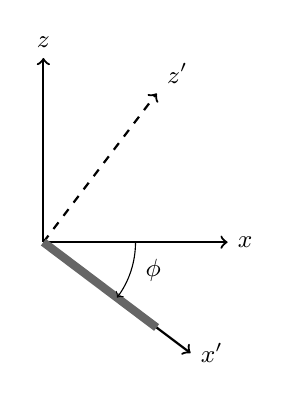
\begin{tikzpicture}[scale=0.9,font=\small]
  \draw[->,thick] (0,0) -- (0,2.6) node[above] {$z$};
  \draw[->,thick] (0,0) -- (2.6,0) node[right] {$x$};
  \draw[->,dashed,thick] (0,0) -- (1.6,2.1) node[above right] {$z'$};
  \draw[line width=3pt,black!60] (0,0) -- (-37:2.0);
  \draw[->,thick] (-37:2.0) -- (-37:2.6) node[right] {$x'$};
  \draw[->] (1.3,0) arc (0:-37:1.3); \node at (1.55,-0.4) {$\phi$};
\end{tikzpicture}

    \end{minipage}
    \begin{equation*}
      \kmat(E,G,I,J,L,\phi) = [T]^\tr[k_l][T] =
      \bmat{1 & 0 & 0\\ 0 & \cos\phi & \sin\phi\\ 0 & -\sin\phi & \cos\phi}
      \begin{bmatrix}\frac{12EI}{L^3} & 0 & \frac{6EI}{L^2}\\[3pt] 0 & \frac{GJ}{L} & 0\\[3pt] \frac{6EI}{L^2} & 0 & \frac{4EI}{L}\end{bmatrix}
      \bmat{1 & 0 & 0\\ 0 & \cos\phi & -\sin\phi\\ 0 & \sin\phi & \cos\phi}
    \end{equation*}
    \begin{equation*}
      \kmat(E,G,I,J,L,\phi) =
      \begin{bmatrix}
        12E\frac{I}{L^3} & 6sE\frac{I}{L^2} & 6cE\frac{I}{L^2}\\[4pt]
        6sE\frac{I}{L^2} & c^2G\frac JL + 4s^2E\frac IL & -scG\frac JL + 4scE\frac IL\\[4pt]
        6cE\frac{I}{L^2} & -scG\frac JL + 4scE\frac IL & s^2G\frac JL + 4c^2E\frac IL
      \end{bmatrix},\qquad c = \cos\phi,\ s = \sin\phi
    \end{equation*}
    \begin{align*}
      ab:\ \rightarrow x'\quad \kmat(29000, 11000, 700, 800, 216, 0) &= \bmat{24.172 & 0 & 2610.6\\ 0 & 40741. & 0\\ 2610.6 & 0 & 3.7593\times10^5}\\
      ae:\ x'\uparrow\quad \kmat(29000, 11000, 700, 800, 120, -0.5\pi) &= \bmat{140.97 & -8458.3 & 0\\ -8458.3 & 6.7667\times10^5 & 0\\ 0 & 0 & 73333.}\\
      ad:\ x'\leftarrow\quad \kmat(29000, 11000, 700, 800, 144, -\pi) &= \bmat{81.581 & 0 & -5873.8\\ 0 & 61111. & 0\\ -5873.8 & 0 & 5.6389\times10^5}\\
      ac:\ x'\downarrow\quad \kmat(29000, 11000, 700, 800, 240, -1.5\pi) &= \bmat{17.622 & 2114.6 & 0\\ 2114.6 & 3.3833\times10^5 & 0\\ 0 & 0 & 36667.}\\
      \text{sum of }[k] &= \bmat{264.35 & -6343.7 & -3263.2\\ -6343.7 & 1.1169\times10^6 & 0\\ -3263.2 & 0 & 1.0498\times10^6}
    \end{align*}
    Note that the sign for $k_{12}$ is different from that given in the textbook. Why?

    \topic{Same example, with the $y$ and $z$ axes the same as those shown in the textbook.}
    \begin{minipage}{0.5\linewidth}
      \begin{equation*}
        [T] = \bmat{1 & 0 & 0\\ 0 & \cos\phi & -\sin\phi\\ 0 & \sin\phi & \cos\phi}
      \end{equation*}
    \end{minipage}\hfill
    \begin{minipage}{0.4\linewidth}\centering
      % Grid: y and z axes as in the textbook (z down)
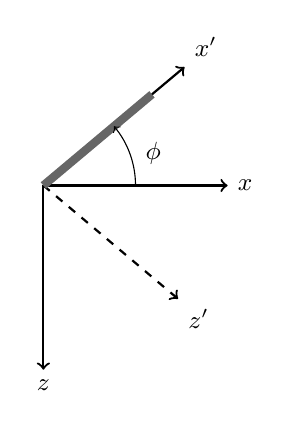
\begin{tikzpicture}[scale=0.9,font=\small]
  \draw[->,thick] (0,0) -- (0,-2.6) node[below] {$z$};
  \draw[->,thick] (0,0) -- (2.6,0) node[right] {$x$};
  \draw[->,dashed,thick] (0,0) -- (1.9,-1.6) node[below right] {$z'$};
  \draw[line width=3pt,black!60] (0,0) -- (40:2.0);
  \draw[->,thick] (40:2.0) -- (40:2.6) node[above right] {$x'$};
  \draw[->] (1.3,0) arc (0:40:1.3); \node at (1.55,0.45) {$\phi$};
\end{tikzpicture}

    \end{minipage}
    \begin{equation*}
      \kmat(E,G,I,J,L,\phi) = [T]^\tr[k_l][T] \quad\text{(same expression as above)}
    \end{equation*}
    \begin{align*}
      ab:\ \rightarrow x'\quad \kmat(29000, 11000, 700, 800, 216, 0) &= \bmat{24.172 & 0 & 2610.6\\ 0 & 40741. & 0\\ 2610.6 & 0 & 3.7593\times10^5}\\
      ae:\ x'\uparrow\quad \kmat(29000, 11000, 700, 800, 120, 0.5\pi) &= \bmat{140.97 & 8458.3 & 0\\ 8458.3 & 6.7667\times10^5 & 0\\ 0 & 0 & 73333.}\\
      ad:\ x'\leftarrow\quad \kmat(29000, 11000, 700, 800, 144, \pi) &= \bmat{81.581 & 0 & -5873.8\\ 0 & 61111. & 0\\ -5873.8 & 0 & 5.6389\times10^5}\\
      ac:\ x'\downarrow\quad \kmat(29000, 11000, 700, 800, 240, 1.5\pi) &= \bmat{17.622 & -2114.6 & 0\\ -2114.6 & 3.3833\times10^5 & 0\\ 0 & 0 & 36667.}\\
      \text{sum of }[k] &= \bmat{264.35 & 6343.7 & -3263.2\\ 6343.7 & 1.1169\times10^6 & 0\\ -3263.2 & 0 & 1.0498\times10^6}
    \end{align*}

  \item \underline{3D truss element, \texttt{ITP}=5}\\
    Degrees of freedom: $\bs{\Delta}^\tr = \langle u_1, v_1, w_1, u_2, v_2, w_2\rangle = \langle 1, 2, 3, 7, 8, 9\rangle$
    \begin{equation*}
      \Tmat = \bmat{\mat{R} & \\ & \mat{R}},\quad\text{with } \mat{R} = \Bmat{\mat{x}'\\ \mat{y}'\\ \mat{z}'},
    \end{equation*}
    where $\mat{x}' = \Bigl\langle\dfrac{x_2-x_1}{L}\ \ \dfrac{y_2-y_1}{L}\ \ \dfrac{z_2-z_1}{L}\Bigr\rangle$; $\mat{y}'$ and $\mat{z}'$ can be any vector. Note that
    \begin{equation*}
      \kmat' = \frac{EA}{L}\bmat{1 & 0 & 0 & -1 & 0 & 0\\ 0 & 0 & 0 & 0 & 0 & 0\\ 0 & 0 & 0 & 0 & 0 & 0\\ -1 & 0 & 0 & 1 & 0 & 0\\ 0 & 0 & 0 & 0 & 0 & 0\\ 0 & 0 & 0 & 0 & 0 & 0}.
    \end{equation*}

  \item \underline{3D frame element, \texttt{ITP}=6}\\
    Degrees of freedom: $\bs{\Delta}^\tr = \langle u_1, v_1, w_1, \theta_{x1}, \theta_{y1}, \theta_{z1}, u_2, v_2, w_2, \theta_{x2}, \theta_{y2}, \theta_{z2}\rangle$
    \begin{equation*}
      \Tmat = \bmat{\mat{R} & & & \\ & \mat{R} & & \\ & & \mat{R} & \\ & & & \mat{R}},\quad\text{with } \mat{R} = \Bmat{\mat{x}'\\ \mat{y}'\\ \mat{z}'}
    \end{equation*}
    where $\mat{x}' = \Bigl\langle\dfrac{x_2-x_1}{L}\ \ \dfrac{y_2-y_1}{L}\ \ \dfrac{z_2-z_1}{L}\Bigr\rangle$, $\mat{y}'$ is the unit vector of one of the principal axes $=$ \texttt{VECTY(3,NBC)} in the program, and $\mat{z}' = \mat{x}'\times\mat{y}'$.

    \begin{minipage}[t]{0.55\linewidth}
      \vspace{0pt}
      Consider a space beam element lying along the $Y$ axis as shown.
      \begin{itemize}
        \item node 1: $(0,0,0)$
        \item node 2: $(0,L,0)$
        \item Therefore, $x' = (0,1,0)$.
      \end{itemize}
    \end{minipage}\hfill
    \begin{minipage}[t]{0.42\linewidth}
      \vspace{0pt}\centering% Space beam element lying along the global Y axis, with four choices of y'
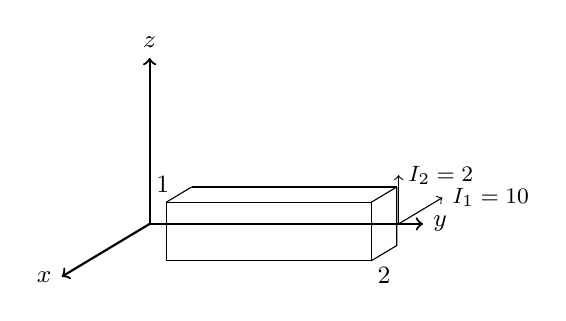
\begin{tikzpicture}[scale=0.62,font=\small,x={(-0.75cm,-0.45cm)},y={(1cm,0cm)},z={(0cm,1cm)}]
  % axes
  \draw[->,thick] (0,0,0) -- (2.4,0,0) node[left] {$x$};
  \draw[->,thick] (0,0,0) -- (0,5.6,0) node[right] {$y$};
  \draw[->,thick] (0,0,0) -- (0,0,3.4) node[above] {$z$};
  % member box from y=0.4 to y=5 with section 0.5 (x) by 1.0 (z)
  \def\ya{0.6} \def\yb{4.8} \def\hx{0.35} \def\hz{0.6}
  \draw (\hx,\ya,\hz) -- (\hx,\yb,\hz) -- (\hx,\yb,-\hz) -- (\hx,\ya,-\hz) -- cycle;
  \draw (-\hx,\ya,\hz) -- (-\hx,\yb,\hz); \draw (\hx,\ya,\hz) -- (-\hx,\ya,\hz); \draw (\hx,\yb,\hz) -- (-\hx,\yb,\hz);
  \draw (-\hx,\yb,\hz) -- (-\hx,\yb,-\hz) -- (\hx,\yb,-\hz);
  \draw[dashed] (0,\ya,0) -- (0,\yb,0);
  \node[left] at (0,\ya,\hz+0.2) {1}; \node[below] at (0,\yb,-\hz-0.1) {2};
  \draw[->] (0,\yb+0.3,0) -- (0,\yb+0.3,1.0) node[right,font=\footnotesize] {$I_2 = 2$};
  \draw[->] (0,\yb+0.3,0) -- (-1.2,\yb+0.3,0) node[right,font=\footnotesize] {$I_1 = 10$};
\end{tikzpicture}

    \end{minipage}

    The following four cases can be distinguished with reference to the selection of the $y'$ axis:
    \begin{align*}
      \text{Case 1: } & y' = (-1,0,0);\ z' = (0,0,1) & (I_{y'},I_{z'}) &= (I_1,I_2) = (10,2)\\
      \text{Case 2: } & y' = (1,0,0);\ z' = (0,0,-1) & (I_{y'},I_{z'}) &= (I_1,I_2) = (10,2)\\
      \text{Case 3: } & y' = (0,0,1);\ z' = (1,0,0) & (I_{y'},I_{z'}) &= (I_2,I_1) = (2,10)\\
      \text{Case 4: } & y' = (0,0,-1);\ z' = (-1,0,0) & (I_{y'},I_{z'}) &= (I_2,I_1) = (2,10)
    \end{align*}
    \begin{fig}
      % Four choices of the local y' axis for a beam along the global Y axis
\begin{tikzpicture}[scale=0.75,font=\small]
  \newcommand{\block}{%
    \draw (0,0) rectangle (0.5,1.2); \draw (0,1.2) -- (-0.6,1.6) -- (-0.1,1.6) -- (0.5,1.2); \draw (-0.6,1.6) -- (-0.6,0.4) -- (0,0);}
  \begin{scope}
    \block
    \draw[->,thick] (0.25,0.6) -- (0.25,2.3) node[above] {$z'$};
    \draw[->,thick] (0.25,0.6) -- (1.9,1.4) node[right] {$y'$};
    \draw[->,thick] (0.25,0.6) -- (1.9,0.1) node[right] {$x'$};
    \node at (0.6,-2.4) {Case 1};
  \end{scope}
  \begin{scope}[xshift=5.2cm]
    \block
    \draw[->,thick] (0.25,0.6) -- (0.25,-1.0) node[below] {$z'$};
    \draw[->,thick] (0.25,0.6) -- (-1.4,-0.2) node[left] {$y'$};
    \draw[->,thick] (0.25,0.6) -- (1.9,0.1) node[right] {$x'$};
    \node at (0.6,-2.4) {Case 2};
  \end{scope}
  \begin{scope}[xshift=10.4cm]
    \block
    \draw[->,thick] (0.25,0.6) -- (0.25,2.3) node[above] {$y'$};
    \draw[->,thick] (0.25,0.6) -- (-1.4,-0.2) node[left] {$z'$};
    \draw[->,thick] (0.25,0.6) -- (1.9,0.1) node[right] {$x'$};
    \node at (0.6,-2.4) {Case 3};
  \end{scope}
  \begin{scope}[xshift=15.6cm]
    \block
    \draw[->,thick] (0.25,0.6) -- (0.25,-1.0) node[below] {$y'$};
    \draw[->,thick] (0.25,0.6) -- (1.9,1.4) node[right] {$z'$};
    \draw[->,thick] (0.25,0.6) -- (1.9,0.1) node[right] {$x'$};
    \node at (0.6,-2.4) {Case 4};
  \end{scope}
\end{tikzpicture}

    \end{fig}
    The global stiffness matrix $\kmat = \Tmat^\tr\kmat'\Tmat$ is the same for the above four cases as expected and is given by
    {\scriptsize
    \begin{equation*}
      \kmat(E,\nu,A,I_1,I_2,J,L) = E\,
      \setlength{\arraycolsep}{1.6pt}
      \begin{bmatrix}
        12\frac{I_2}{L^3} & 0 & 0 & 0 & 0 & -6\frac{I_2}{L^2} & -12\frac{I_2}{L^3} & 0 & 0 & 0 & 0 & -6\frac{I_2}{L^2}\\[3pt]
        0 & \frac AL & 0 & 0 & 0 & 0 & 0 & -\frac AL & 0 & 0 & 0 & 0\\[3pt]
        0 & 0 & 12\frac{I_1}{L^3} & 6\frac{I_1}{L^2} & 0 & 0 & 0 & 0 & -12\frac{I_1}{L^3} & 6\frac{I_1}{L^2} & 0 & 0\\[3pt]
        0 & 0 & 6\frac{I_1}{L^2} & 4\frac{I_1}{L} & 0 & 0 & 0 & 0 & -6\frac{I_1}{L^2} & 2\frac{I_1}{L} & 0 & 0\\[3pt]
        0 & 0 & 0 & 0 & \frac12\frac{J}{(1+\nu)L} & 0 & 0 & 0 & 0 & 0 & -\frac12\frac{J}{(1+\nu)L} & 0\\[3pt]
        -6\frac{I_2}{L^2} & 0 & 0 & 0 & 0 & 4\frac{I_2}{L} & 6\frac{I_2}{L^2} & 0 & 0 & 0 & 0 & 2\frac{I_2}{L}\\[3pt]
        -12\frac{I_2}{L^3} & 0 & 0 & 0 & 0 & 6\frac{I_2}{L^2} & 12\frac{I_2}{L^3} & 0 & 0 & 0 & 0 & 6\frac{I_2}{L^2}\\[3pt]
        0 & -\frac AL & 0 & 0 & 0 & 0 & 0 & \frac AL & 0 & 0 & 0 & 0\\[3pt]
        0 & 0 & -12\frac{I_1}{L^3} & -6\frac{I_1}{L^2} & 0 & 0 & 0 & 0 & 12\frac{I_1}{L^3} & -6\frac{I_1}{L^2} & 0 & 0\\[3pt]
        0 & 0 & 6\frac{I_1}{L^2} & 2\frac{I_1}{L} & 0 & 0 & 0 & 0 & -6\frac{I_1}{L^2} & 4\frac{I_1}{L} & 0 & 0\\[3pt]
        0 & 0 & 0 & 0 & -\frac12\frac{J}{(1+\nu)L} & 0 & 0 & 0 & 0 & 0 & \frac12\frac{J}{(1+\nu)L} & 0\\[3pt]
        -6\frac{I_2}{L^2} & 0 & 0 & 0 & 0 & 2\frac{I_2}{L} & 6\frac{I_2}{L^2} & 0 & 0 & 0 & 0 & 4\frac{I_2}{L}
      \end{bmatrix}
    \end{equation*}}
\end{enumerate}
